\chapter[Resultados e discussão]{Resultados e discussão}


% RESULTADOS: 
% Discutir/analisar o código
% Criar logs de simulação
% Mostrar a tela do aplicativo

\section{Análise do código}
\subsection{Comunicação Bluetooth}

A comunicação entre o firmware e o aplicativo é realizada por meio da tecnologia BLE, a qual impõe uma limitação significativa: cada pacote transmitido ou recebido possui um tamanho máximo de 20 bytes. Com base nessa restrição, o código foi estruturado de forma a otimizar o uso dos pacotes disponíveis, minimizando a quantidade de transmissões necessárias e, consequentemente, aumentando a eficiência da comunicação.

Para isso, optou-se por transmitir dados diretamente no formato \texttt{byte}, o que permite o envio de até 20 valores distintos em um único pacote. Essa abordagem, no entanto, limita os valores possíveis ao intervalo de 0 a 255, conforme a representação padrão de um byte. Em situações onde foi necessário ultrapassar esse limite, foi implementada uma lógica de fragmentação dos dados, permitindo a representação de valores mais elevados por meio da combinação de dois ou mais bytes. Com esse método, tornou-se possível transmitir qualquer número, com precisão suficiente para valores decimais simples.

Essa lógica foi aplicada, por exemplo, na transmissão da informação referente ao percentual de uso da memória RAM, que exige a representação de números com casas decimais. Nessa aplicação específica, o valor percentual é multiplicado por 100 e, em seguida, dividido em dois bytes para envio, sendo reconstituído com a operação inversa no aplicativo receptor (\autoref{fig:sendheartbeat}).

\begin{figure}[ht]
    \centering
    \caption{Função assíncrona do envio do sinal periódico de conexão com envio fragmentado da memória utilizada pelo dispositivo.}
    \label{fig:sendheartbeat}
    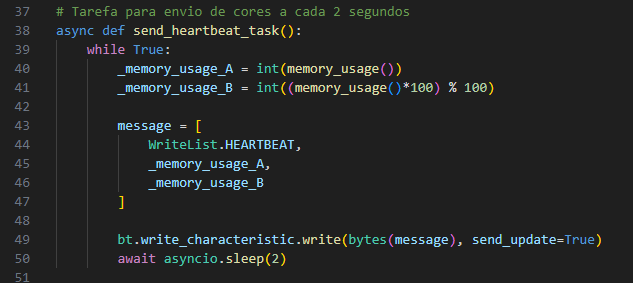
\includegraphics[width=1.0\textwidth]{5_sendheartbeat.png}

    {\centering\footnotesize Fonte: Autoria própria.\par}
\end{figure}

A estratégia de triagem dos dados recebidos parte da utilização do primeiro byte do pacote como identificador, permitindo a categorização e o encaminhamento adequado de cada mensagem. Para facilitar essa operação e melhorar a legibilidade do código, foram implementadas duas classes – \texttt{ReadList} e \texttt{WriteList} – que reservam os 256 valores possíveis para identificadores (\autoref{fig:classreadlist}). Essa abordagem permite que cada valor atribuído seja mapeado a uma ação específica, otimizando o fluxo de comunicação entre o firmware e o aplicativo.

Para exemplificar, na função \texttt{def send\_heartbeat\_task()} (\autoref{fig:sendheartbeat}), a variável \texttt{message} representa um array construído por meio da classe \texttt{WriteList}, de onde é extraído o identificador correspondente. Este identificador é utilizado no aplicativo receptor para direcionar o tratamento da mensagem, garantindo a correta interpretação dos dados enviados.

\begin{figure}[ht]
    \centering
    \caption{Declaração das classes de constantes dos identificadores de pacotes.}
    \label{fig:classreadlist}
    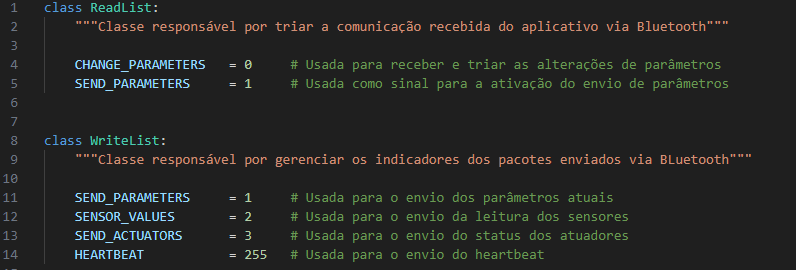
\includegraphics[width=1.0\textwidth]{5_identificadores_com.png}

    {\centering\footnotesize Fonte: Autoria própria.\par}
\end{figure}

A lógica de comunicação implementada no aplicativo Android segue o mesmo princípio de identificação adotado no firmware. O primeiro byte do pacote recebido é utilizado como identificador, sendo interpretado para direcionar o tratamento adequado dos dados (\autoref{fig:onreadupdate}). Por exemplo, quando esse identificador assume o valor 255, entende-se que o pacote refere-se ao sinal de \textit{heartbeat} enviado periodicamente pelo ESP32, contendo também o percentual de uso da memória RAM (\autoref{fig:condicionaldereceberusodememoria}).

\begin{figure}[ht]
    \centering
    \caption{Trecho do código do aplicativo que mostra a triagem dos dados recebidos.}
    \label{fig:onreadupdate}
    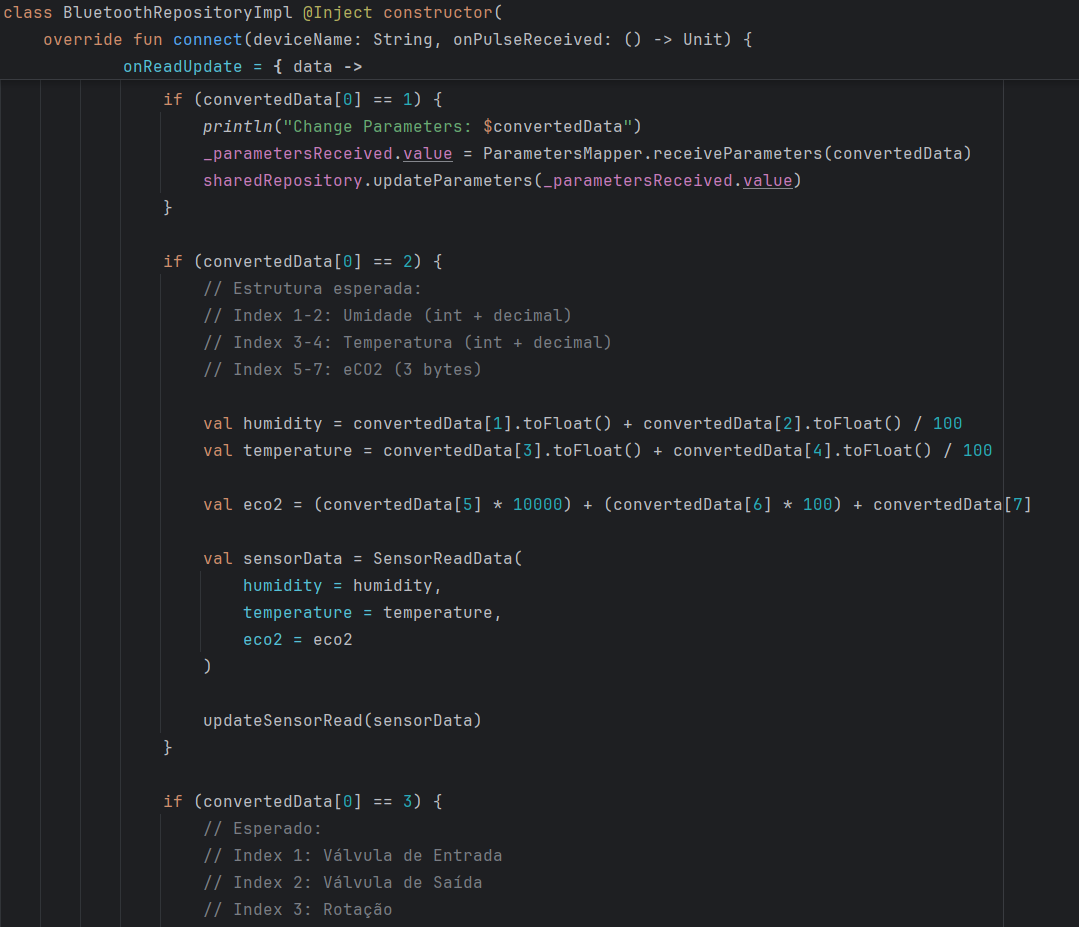
\includegraphics[width=1.0\textwidth]{5_onreadupdate.png}

    {\centering\footnotesize Fonte: Autoria própria.\par}
\end{figure}

\begin{figure}[ht]
    \centering
    \caption{Trecho do código do aplicativo que mostra o tratamento do pacote identificado com 255.}
    \label{fig:condicionaldereceberusodememoria}
    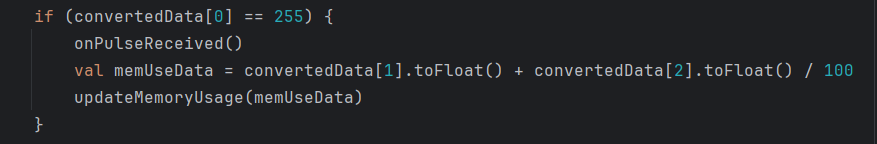
\includegraphics[width=1.0\textwidth]{5_condicionaldereceberusodememoria.png}

    {\centering\footnotesize Fonte: Autoria própria.\par}
\end{figure}


Nesse contexto, o aplicativo interpreta os bytes seguintes como valores numéricos que representam, respectivamente, a parte inteira e a parte decimal da porcentagem. Esses valores são somados após a conversão para o formato numérico adequado, resultando em um valor final com duas casas decimais (\autoref{fig:condicionaldereceberusodememoria}). Esse número é então utilizado para atualizar a interface do usuário com a informação atualizada sobre o consumo de memória do dispositivo.

Além da extração dos dados de uso de memória, o recebimento do identificador 255 também aciona uma função interna responsável por sinalizar a chegada do \textit{heartbeat}. Esse mecanismo funciona como um pulso periódico enviado pelo firmware, cuja função principal é indicar que o dispositivo segue ativo e em comunicação com o aplicativo. No aplicativo, esse pulso ativa um recurso visual na interface: uma indicação em forma de círculo que pisca a cada novo recebimento. Esse indicador atua como um monitor de conexão em tempo real, permitindo ao usuário verificar de forma intuitiva se a comunicação Bluetooth está estável. Caso o pulso deixe de ser recebido por um intervalo prolongado, o usuário deve observar que ocorreu a perda de sinal ou falha de comunicação, evitando a falsa impressão de que o sistema permanece operacional quando, na verdade, pode estar congelado ou desconectado.

Esse modelo de tratamento baseado em identificadores garante clareza na separação das funções e facilita futuras expansões, mantendo o código modular e de fácil manutenção.


\subsection{Parâmetros de malteação}

Os parâmetros de malteação são definidos no sistema como todas as variáveis que o malteador deve controlar ao longo do processo. No firmware, esses parâmetros são declarados como variáveis globais no arquivo \texttt{init\_data.py} (\autoref{fig:initparameters}), garantindo que estejam acessíveis em diferentes partes do sistema.

\begin{figure}[ht]
    \centering
    \caption{Algoritmo de inicialização dos parâmetros.}
    \label{fig:initparameters}
    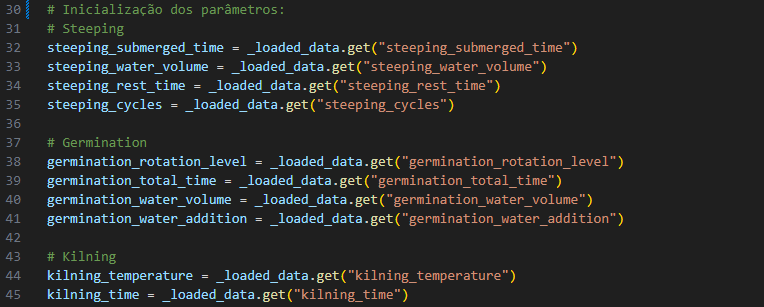
\includegraphics[width=1.0\textwidth]{5_initparameters.png}

    {\centering\footnotesize Fonte: Autoria própria.\par}
\end{figure}

Durante a inicialização do ESP32, os valores desses parâmetros são carregados do arquivo \texttt{config.json}. Os dados são primeiramente lidos e armazenados na variável local \texttt{\_loaded\_data} e, em seguida, os valores são distribuídos para as respectivas variáveis globais, configurando o sistema com a última configuração salva (\autoref{fig:initparameters}).

Ainda nesse mesmo módulo (\texttt{init\_data.py}), existe uma função dedicada à reescrita do arquivo \texttt{config.json} com novos valores fornecidos pelo usuário (\autoref{fig:defrewrite}). Essa função permite que, ao receber novos parâmetros via comunicação Bluetooth, o firmware atualize o arquivo de configuração de forma persistente. Com isso, é possível modificar os parâmetros diretamente pelo aplicativo, garantindo que essas alterações permaneçam salvas mesmo após desligamentos ou reinicializações do sistema.

\begin{figure}[ht]
    \centering
    \caption{Algoritmo de salvamento dos parâmetros recebidos.}
    \label{fig:defrewrite}
    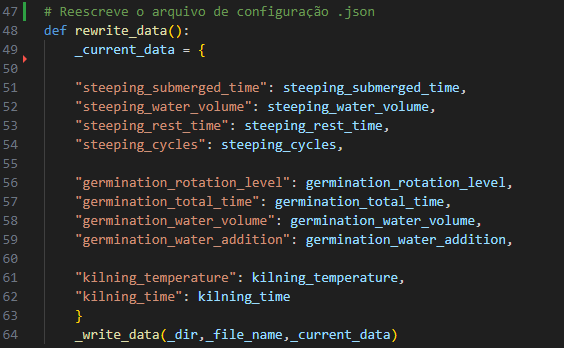
\includegraphics[width=0.8\textwidth]{5_defrewrite.png}

    {\centering\footnotesize Fonte: Autoria própria.\par}
\end{figure}

Os parâmetros de malteação foram otimizados para que seus valores pudessem ser representados dentro da faixa de um único byte, permitindo até 256 variações distintas por parâmetro. Essa decisão buscou equilibrar a precisão necessária para o controle do processo com a eficiência na comunicação via Bluetooth, já que o envio de todos os parâmetros em um único pacote reduz o tempo de transmissão e garante que não ocorrerá perda de pacotes, caso que precisaria ser tratado.

Embora essa abordagem limite os valores possíveis, ela se mostra adequada frente às grandezas envolvidas do processo. Caso, em fases futuras de otimização do malteador, seja identificada a necessidade de uma resolução mais fina para algum parâmetro específico, a estrutura atual do sistema permite, de forma simples, a adição de bytes extras para ampliar a faixa de representação dos valores, sem impacto significativo na arquitetura dos módulos existentes. No entanto, considerando os intervalos típicos de operação, não se espera que essa expansão seja necessária.

\begin{figure}[ht]
    \caption{Parâmetros de correção de valores para otimização da comunicação Bluetooth.}
    \label{fig:parameterscorrections}
    \centering
    \subfloat[Maceração\label{subfig:correctiona}]{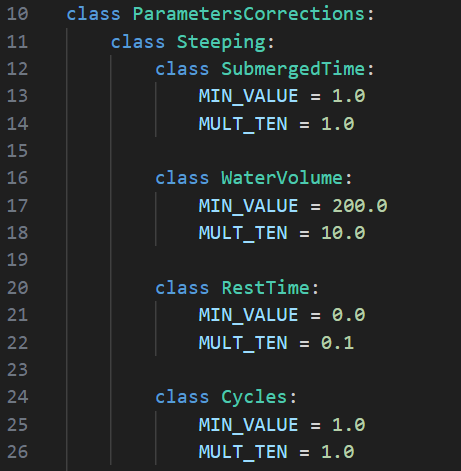
\includegraphics[width=0.3\textwidth]{5_corrections_a.png}}
    \hfill
    \subfloat[Germinação\label{subfig:correctionb}]{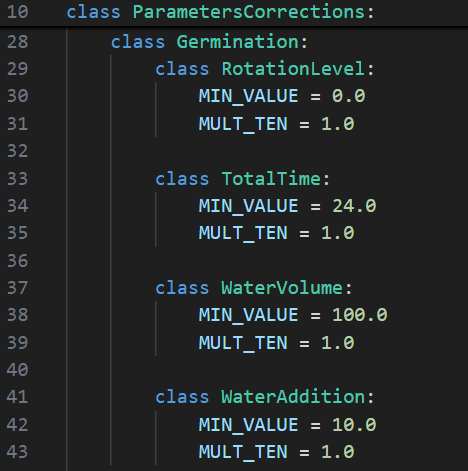
\includegraphics[width=0.3\textwidth]{5_corrections_b.png}}
    \hfill
    \subfloat[Secagem\label{subfig:correctionc}]{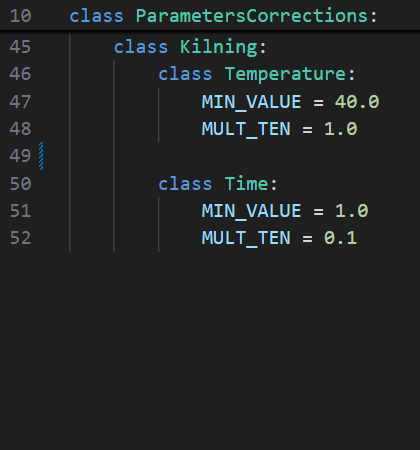
\includegraphics[width=0.28\textwidth]{5_corrections_c.png}}

    {\centering\footnotesize Fonte: Autoria própria.\par}

\end{figure}

A \autoref{fig:parameterscorrections} apresenta os fatores de correção utilizados para conversão dos valores dos parâmetros tanto no envio quanto no recebimento. Ao receber um novo conjunto de configurações o valor bruto do byte referente ao parâmetro é multiplicado por uma constante de escala (\texttt{MULT\_TEN}) e somado ao valor mínimo admissível (\texttt{MIN\_VALUE}), garantindo que a faixa de operação seja respeitada. Esse tratamento é aplicado na função responsável pela alteração dos parâmetros recebidos, conforme ilustrado na \autoref{fig:changeparameters}. A operação inversa é realizada quando se cria um pacote de envio dos parâmetros atuais através da solicitação do aplicativo.

Na \autoref{tab:parametros}, são listados todos os parâmetros disponíveis no sistema, acompanhados de suas respectivas faixas de valores operacionais, definidas conforme os limites estabelecidos.

\begin{figure}[ht]
    \centering
    \caption{Trecho da função assíncrona de alteração dos parâmetros.}
    \label{fig:changeparameters}
    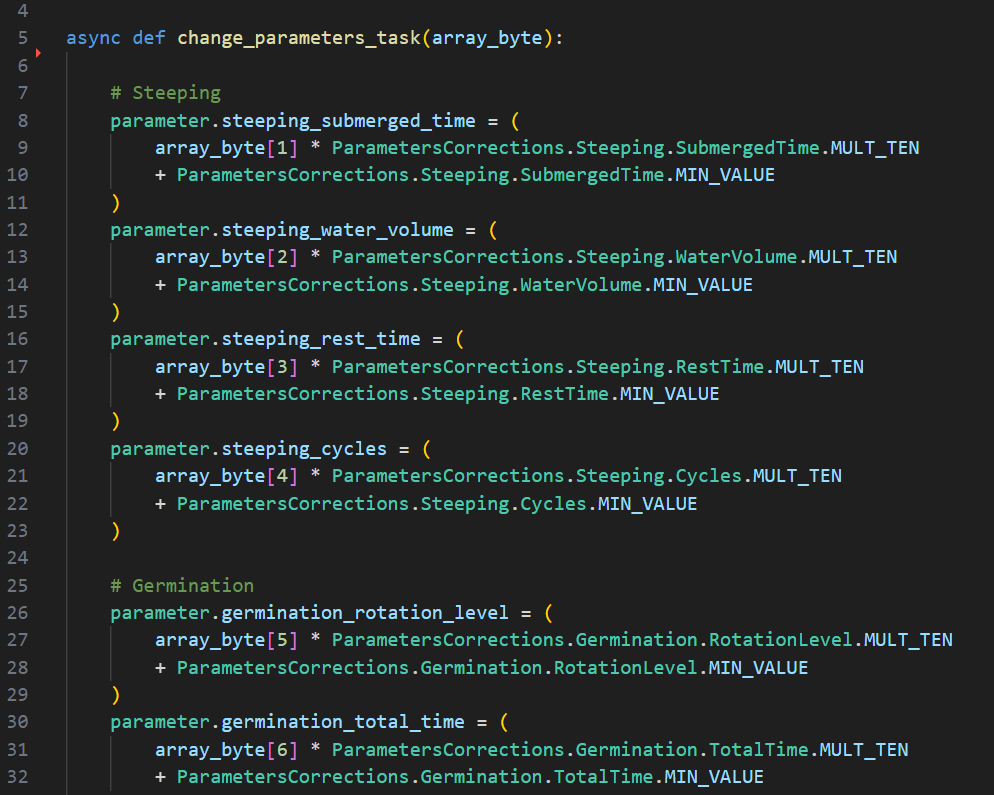
\includegraphics[width=0.9\textwidth]{5_changeparameters.png}

    {\centering\footnotesize Fonte: Autoria própria.\par}
\end{figure}

\begin{table}[ht]
    \caption{Faixa de valores possíveis para cada parâmetro.}
    \label{tab:parametros}
    \centering
    \begin{tabular}{cccc}
        \hline
        \bfseries Parâmetro & \bfseries Etapa & \bfseries Faixa de Valores & \bfseries Unidade \\
        \hline
        Tempo Submerso & Maceração & 1 -- 256  & horas \\
        Volume de Água & Maceração & 200 -- 2750 & mL \\
        Tempo de Descanso & Maceração & 0.0 -- 25,5 & horas \\
        Número de Ciclos & Maceração & 1 -- 256 & ciclos \\
        Nível de Rotação & Germinação & 0 -- 255 & -- \\
        Tempo Total & Germinação & 24 -- 279 & horas \\
        Volume de Água & Germinação & 100 -- 355 & mL \\
        Adição de Água & Germinação & 10 -- 265 & minutos \\
        Temperatura & Secagem & 40 -- 295 & $^{\circ}$C \\
        Tempo Total & Secagem & 1.0 -- 26.5 & horas \\
        \hline
    \end{tabular}

    {\centering\footnotesize Fonte: Autoria própria.\par}
\end{table}



\subsection{Algoritmo da malteação}

A estrutura do algoritmo de malteação foi desenvolvida com base em um modelo assíncrono, utilizando tarefas concorrentes para controlar diferentes aspectos do processo de forma simultânea. A lógica principal se dá na função que gerencia o ciclo completo da malteação (\autoref{fig:executemalting}), ativada quando o sistema recebe o comando de início por meio do aplicativo. Esse controle é feito com base em uma estrutura de estado global (\autoref{fig:maltingcontrol}), que registra o estágio atual do processo e permite a interrupção imediata por meio de um sinal de aborto.

\begin{figure}[ht]
    \centering
    \caption{Função assíncrona para o gerenciamento da malteação.}
    \label{fig:executemalting}
    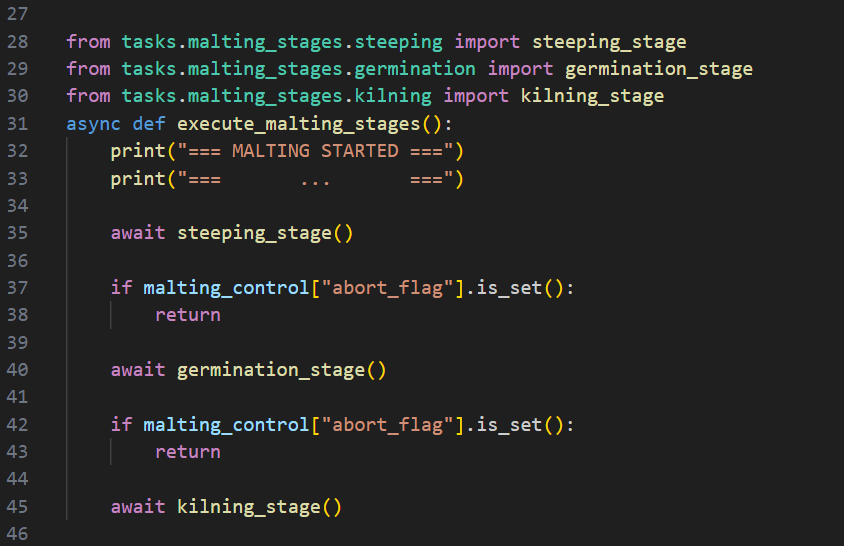
\includegraphics[width=0.9\textwidth]{5_executemalting.png}

    {\centering\footnotesize Fonte: Autoria própria.\par}
\end{figure}

\begin{figure}[ht]
    \centering
    \caption{Estado global do status da malteação.}
    \label{fig:maltingcontrol}
    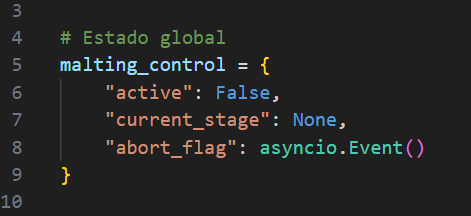
\includegraphics[width=0.8\textwidth]{5_maltingcontrol.png}

    {\centering\footnotesize Fonte: Autoria própria.\par}
\end{figure}

\subsubsection{Maceração}

A primeira etapa executada após o acionamento do sistema é a maceração. Ao entrar nesse estágio, o sistema atualiza o estado global para refletir a fase ativa (\textit{steeping}) e inicia duas tarefas assíncronas em paralelo: uma para controle de temperatura e outra para execução dos ciclos de tempo (\autoref{fig:steepingstage}). Essa separação permite que o sistema monitore e regule a temperatura de forma contínua, sem interromper a sequência temporal dos ciclos de hidratação.

\begin{figure}[ht]
    \centering
    \caption{Função assíncrona da maceração.}
    \label{fig:steepingstage}
    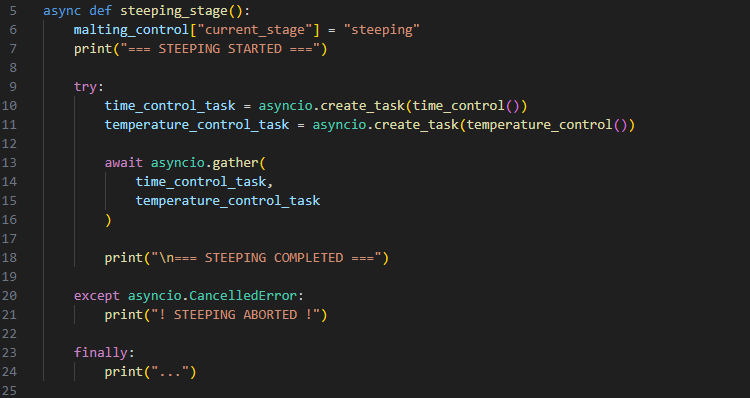
\includegraphics[width=1.0\textwidth]{5_steepingstage.png}

    {\centering\footnotesize Fonte: Autoria própria.\par}
\end{figure}

Durante o controle de tempo, são executadas, de forma sequencial, as quatro subetapas que compõem cada ciclo de \textit{steeping}: enchimento do recipiente, imersão dos grãos, drenagem da água e repouso (\autoref{fig:timesteeping}). Cada uma dessas fases é monitorada individualmente, e interrupções podem ser feitas a qualquer momento caso o sinal de aborto seja detectado. Esse comportamento é implementado por meio de verificações constantes dentro dos \textit{loops}, garantindo que o processo possa ser interrompido de forma imediata.

\begin{figure}[ht]
    \centering
    \caption{Função assíncrona do controle de tempo da maceração.}
    \label{fig:timesteeping}
    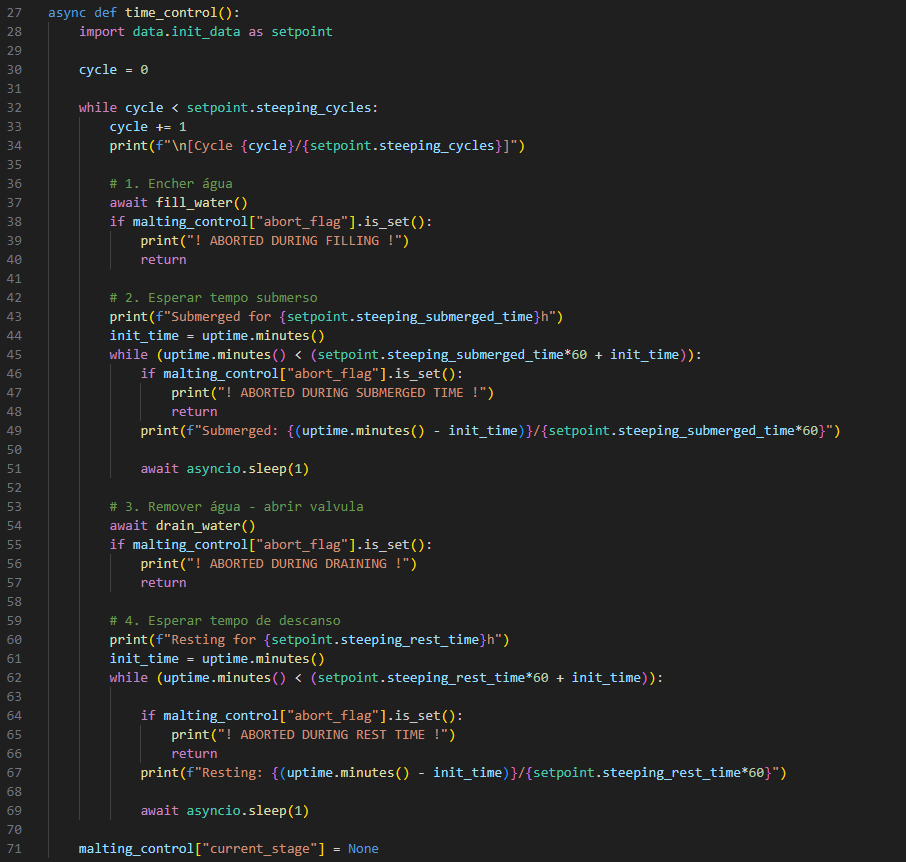
\includegraphics[width=1.0\textwidth]{5_timesteeping.png}

    {\centering\footnotesize Fonte: Autoria própria.\par}
\end{figure}

O controle de válvulas, tanto para enchimento quanto para drenagem, segue um modelo baseado no tempo de abertura, adicionando o volume necessário para a operação. Apesar de simplificado, esse método pode ser ajustado posteriormente com base em calibrações que relacionem diretamente o tempo de válvula aberta ao volume de água processado. Esse aspecto é fundamental para permitir futuras melhorias sem a necessidade de reescrita da estrutura de controle.

A lógica de controle de temperatura já está inserida como uma tarefa paralela com checagens periódicas e resposta ao sinal de aborto, embora o controle de temperatura (resfriamento) ainda não seja possível de controlar no ESP32 devido às características do protótipo desenolvido na IC. Essa estrutura modular (\autoref{fig:temperaturecontrol}) permite que, posteriormente, os sensores e atuadores sejam integrados com precisão ao algoritmo principal, mantendo a arquitetura atual.

\begin{figure}[ht]
    \centering
    \caption{Função assíncrona que simula o controle de temperatura (resfriamento).}
    \label{fig:temperaturecontrol}
    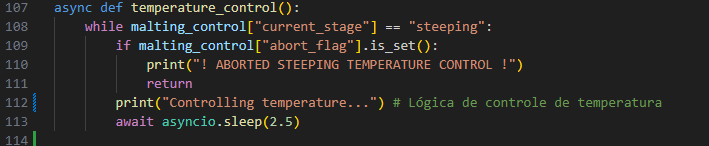
\includegraphics[width=0.8\textwidth]{5_temperaturecontrol.png}

    {\centering\footnotesize Fonte: Autoria própria.\par}
\end{figure}

Ao final da execução dos ciclos de macaeração, o sistema limpa o estado da etapa atual (linha 71 na \autoref{fig:timesteeping}) e aguarda a próxima fase do processo.

\subsubsection{Germinação}

A etapa de germinação (\textit{germination}) dá continuidade ao processo. Assim como na etapa anterior, a estrutura do algoritmo é dividida em tarefas paralelas que atuam de maneira cooperativa para garantir o andamento e a estabilidade do processo. Ao iniciar a germinação, o sistema atualiza o estado global e ativa quatro tarefas assíncronas simultâneas: controle de tempo, temperatura, umidade e rotação (\autoref{fig:germinationstage}).

\begin{figure}[ht]
    \centering
    \caption{Função assíncrona da germinação.}
    \label{fig:germinationstage}
    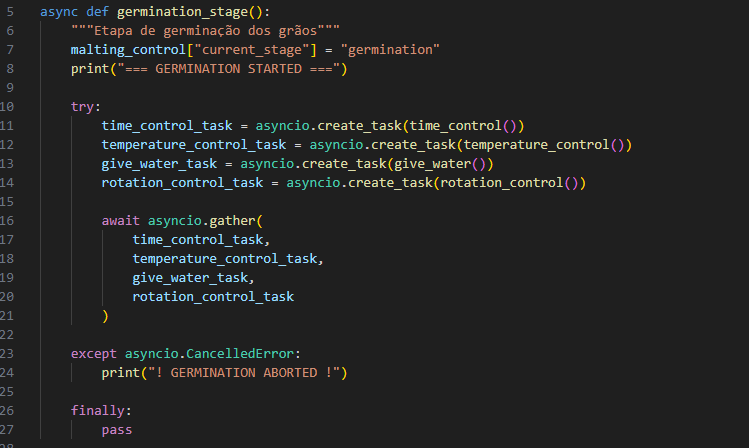
\includegraphics[width=0.8\textwidth]{5_germinationstage.png}

    {\centering\footnotesize Fonte: Autoria própria.\par}
\end{figure}

O controle temporal da germinação consiste em um cronômetro contínuo que delimita o tempo total da etapa com base nos parâmetros definidos. Essa tarefa funciona como base para as demais, mantendo o sistema ativo durante todo o ciclo da germinação e sinalizando o encerramento do estágio quando o tempo total é atingido. Ao longo desse intervalo, as outras variáveis são mantidas sob controle (\autoref{fig:germinationtimecontrol}).

\begin{figure}[ht]
    \centering
    \caption{Função assíncrona de controle de tempo da germinação.}
    \label{fig:germinationtimecontrol}
    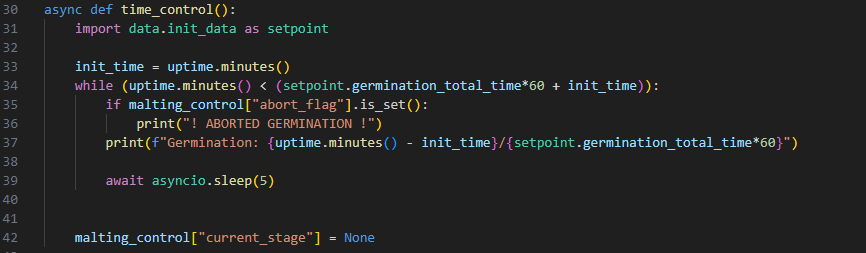
\includegraphics[width=1.0\textwidth]{5_germinationtimecontrol.png}

    {\centering\footnotesize Fonte: Autoria própria.\par}
\end{figure}

A umidificação periódica dos grãos é feita por meio de ciclos adicionam de água. O algoritmo alterna entre a abertura de válvulas para umidificar o ambiente e pausas programadas para não encharcar os grãos. Essa tarefa permanece ativa enquanto o estágio estiver em execução, repetindo os ciclos conforme o necessário. O controle de temperatura segue o mesmo princípio adotado na etapa anterior, sendo executado como tarefa independente que verifica periodicamente o estado do sistema, permitindo ajustes térmicos futuros.

Além disso, durante a germinação, o sistema realiza rotações constantes, para o revolvimento dos grãos com o objetivo de garantir a aeração e evitar o emaranhamento das radículas. Toda a estrutura da germinação foi desenvolvida para funcionar com a verificação constante do estado de abortamento.

\subsubsection{Secagem}

Encerrada a germinação, inicia-se a última etapa do processo: a secagem (\textit{kilning}). Nesta fase, o objetivo é reduzir a umidade dos grãos e interromper a atividade enzimática, preservando as características desejadas do malte. A lógica geral da secagem mantém o padrão das etapas anteriores, utilizando tarefas assíncronas paralelas para controle de tempo, temperatura e rotação (\autoref{fig:kilning}).

\begin{figure}[ht]
    \centering
    \caption{Função assíncrona da secagem.}
    \label{fig:kilning}
    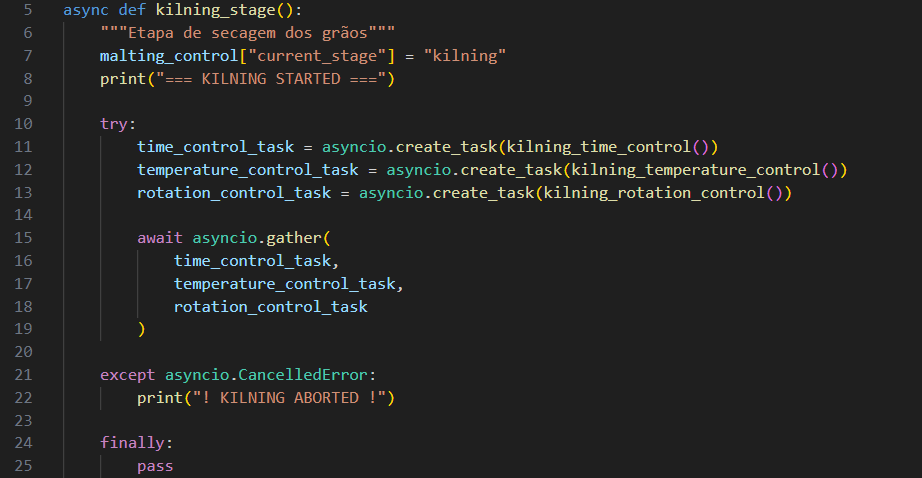
\includegraphics[width=1.0\textwidth]{5_kilning.png}

    {\centering\footnotesize Fonte: Autoria própria.\par}
\end{figure}

O controle de tempo define a duração total do estágio, monitorando continuamente a contagem regressiva com base nos parâmetros definidos pelo usuário (linha 11 da \autoref{fig:kilning}). Já a temperatura, nesse estágio, assume papel ainda mais crítico, visto que a secagem envolve temperaturas elevadas e potencialmente danosas ao produto se não forem adequadamente controladas.

Por fim, o controle de rotação continua presente (linha 13 da \autoref{fig:kilning}), com o intuito de garantir a homogeneidade da secagem e evitar a formação de zonas com retenção de umidade. Essa movimentação periódica dos grãos deve assegurar uma secagem eficiente e uniforme.

A estrutura assíncrona aplicada em todas as etapas da malteação permite ao sistema operar com múltiplos controles simultâneos, com segurança, responsividade e flexibilidade. A separação lógica das funções facilita tanto a manutenção do código quanto a sua expansão, criando uma base para futuras implementações automatizadas, como a inclusão de um programa de torra.

\subsection{Sensores e Atuadores}

Nesta implementação, foram utilizados dois sensores conectados via protocolo I\textsuperscript{2}C: o \textbf{AHT20}, responsável pela medição de temperatura e umidade relativa, e o \textbf{ENS160}, sensor digital de qualidade do ar, empregado aqui para leitura do valor de eCO\textsubscript{2} (equivalente de dióxido de carbono). Ambos os sensores foram instanciados e gerenciados no módulo \texttt{sensor\_reader.py}, onde é realizada a leitura cíclica dos dados ambientais por meio da função \texttt{get\_sensor\_readings()} (\autoref{fig:sensorreader}).

\begin{figure}[ht]
    \centering
    \caption{Módulo de leitura dos sensores.}
    \label{fig:sensorreader}
    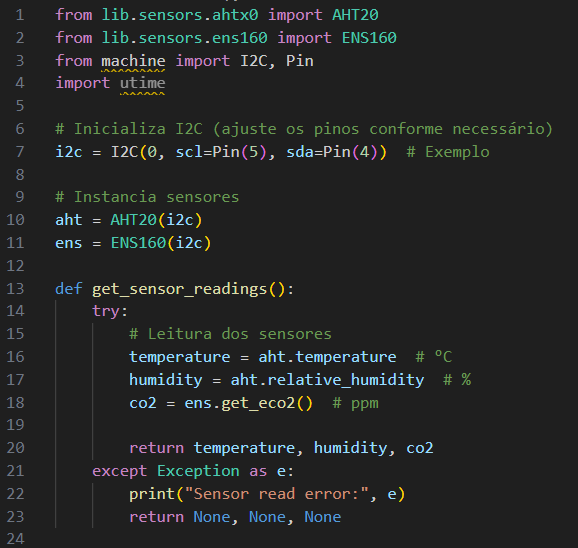
\includegraphics[width=1.0\textwidth]{5_sensorreader.png}

    {\centering\footnotesize Fonte: Autoria própria.\par}
\end{figure}

A leitura dos sensores ocorre de maneira contínua e assíncrona na tarefa \texttt{sensors\_task()} (\autoref{fig:sensorstask}), garantindo atualização constante dos dados. Após cada leitura, os valores de temperatura, umidade e eCO\textsubscript{2} são armazenados em variáveis globais do dicionário \texttt{sensor\_values}, facilitando o acesso por outras tarefas do sistema. Para fins de transmissão Bluetooth, os valores são convertidos em bytes e enviados periodicamente para o aplicativo dentro dessa própria função.

\begin{figure}[ht]
    \centering
    \caption{Trecho da função assíncrona de leitura dos sensores.}
    \label{fig:sensorstask}
    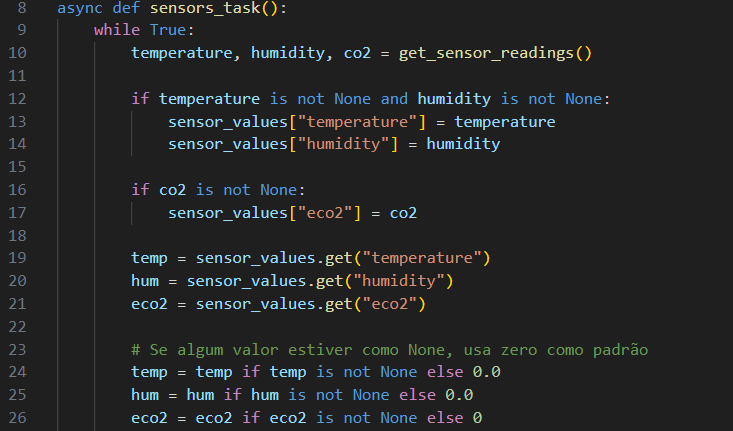
\includegraphics[width=1.0\textwidth]{5_sensorstask.png}

    {\centering\footnotesize Fonte: Autoria própria.\par}
\end{figure}

O tratamento de falhas também foi considerado: caso a leitura de qualquer sensor falhe, o sistema atribui valor zero como padrão, garantindo que o fluxo da comunicação continue sem interrupções.

Em paralelo à leitura de sensores, o sistema também gerencia cinco atuadores principais: duas válvulas (entrada e saída de água), um motor de rotação, uma resistência térmica e uma bomba de ar. A lógica de controle desses dispositivos é encapsulada na classe \texttt{Actuator} (\autoref{fig:actuatorclass}), desenvolvida para simplificar a manipulação dos pinos GPIO e abstrair as diferenças de lógica de acionamento (ativo-alto ou ativo-baixo).

\begin{figure}[ht]
    \centering
    \caption{Definição da classe \texttt{Actuator}.}
    \label{fig:actuatorclass}
    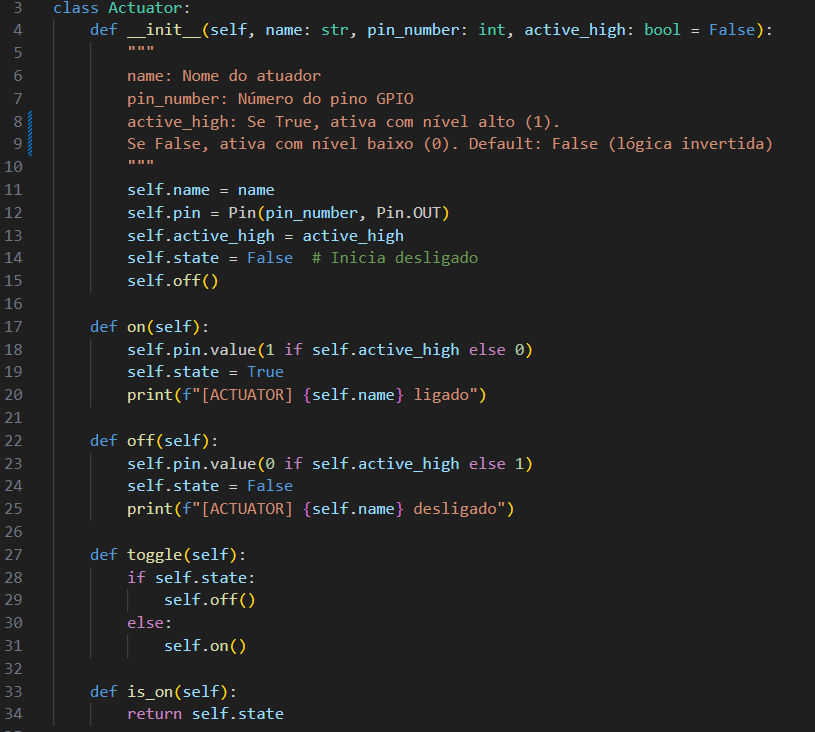
\includegraphics[width=1.0\textwidth]{5_actuatorclass.png}

    {\centering\footnotesize Fonte: Autoria própria.\par}
\end{figure}

Cada atuador é instanciado em \texttt{actuators.py} com seu respectivo nome e número de pino, e armazenado em um dicionário global para facilitar o acesso dinâmico por outras partes do sistema (\autoref{fig:actuatorsdata}). A classe disponibiliza métodos como \texttt{on()}, \texttt{off()} e \texttt{toggle()}, além de uma função de verificação de estado atual. Dessa forma, o acionamento de cada dispositivo torna-se simples, confiável e rastreável (via terminal).

\begin{figure}[ht]
    \centering
    \caption{Módulo de gerenciamento dos atuadores.}
    \label{fig:actuatorsdata}
    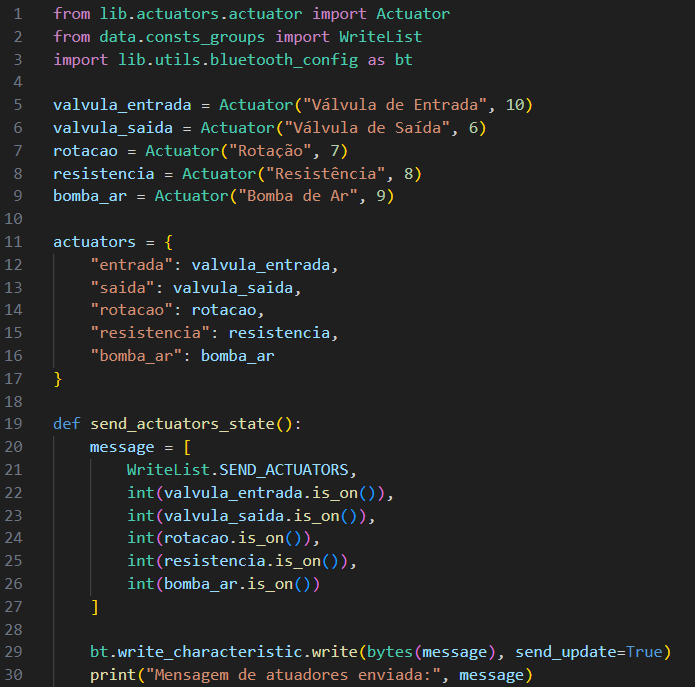
\includegraphics[width=1.0\textwidth]{5_actuatorsdata.png}

    {\centering\footnotesize Fonte: Autoria própria.\par}
\end{figure}

Além do controle direto, foi implementada uma função de envio do estado atual dos atuadores via Bluetooth, permitindo que o aplicativo visualize, em tempo real, quais dispositivos estão ativos no momento (linha 19 na \autoref{fig:actuatorsdata}).

\section{Aplicativo Android}
